\section{Theorie}
\label{sec:Theorie}

% In knapper Form sind die physikalischen Grundlagen des Versuches, des Messverfahrens, sowie sämtliche für die Auswertung erforderlichen Gleichungen darzustellen. (Keine Herleitung)

% (eventuell die Aufgaben)

% Der Versuchsaufbau: Beschreibung des Versuchs und der Funktionsweise (mit Skizze/Bild/Foto)
 
Für diesen Versuch wird Licht als elektromagnetische Welle der Form 
\begin{equation}
    \vec{E}(x,t) = \vec{E_0} \cdot \cos{\left(k \cdot x - \omega \cdot t - \delta\right)}
    \label{eq:licht}
\end{equation}
angenommen. 
Der Teilchencharakter von Licht wird hier ignoriert.
Hierbei ist $k$ die Wellenzahl, $\omega$ die Kreisfrequenz und $\delta$ der Phasenwinkel.
Die Intensität $I$ einer solchen Welle lässt sich über 
\begin{equation}
    I = c \cdot |\vec{E_0}|^2
\end{equation}
berechnen, mit der Konstante $c$.
Werden zwei Wellen dieser Art überlagert, ergibt sich die folgende Gesamtintensität
\begin{equation}
    I_\text{ges} = 2\cdot c \cdot \vec{E_0}^2 \left(1 + \cos{(\delta_2 - \delta_1)}\right)
\end{equation}
Es ist zu beobachten, dass sich die Wellenintensitäten nicht einfach addieren, sondern ein sogenannter Interferenzterm $2\cdot c \cdot \vec{E_0}^2\cos{(\delta_2 - \delta_1)}$ addiert werden muss.
Durch die Eigenschaften des Cosinus ergibt sich, dass die Gesamtintensität verschwindet, wenn $\delta_2 - \delta_1$ ein ungerades Vielfaches von $\pi$ ist.

Um diesen Interferenzeffekt beobachten können, muss kohärentes Licht verwendet werden.
Also Licht dessen Wellen sich nach \autoref{eq:licht} verhalten. 
Ein Laser erfüllt diese Bedingung, denn $k$, $\omega$ und $\delta$ sind bei jeder Welle nahezu gleich. 
Überlicherweise wird für die Beobachtung der Interferenzeffekte ein einzelner Laser verwendet, dieser wird wie in \autoref{fig:bild1} in zwei Strahlen aufgeteilt und teilweise umgelenkt.
Wenn die beiden Strahlen wieder gebündelt werden, haben sie eine Phasenverschiebung untereinander.

\begin{figure}
    \centering
    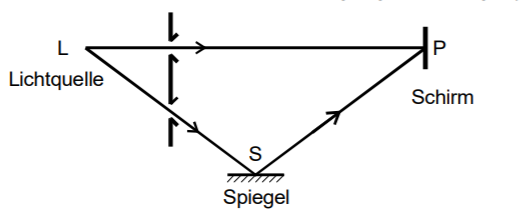
\includegraphics[width=0.4\textwidth]{images/bild1.png}
    \caption{Prinzip der Phasenverschiebung.\cite{V401}}
    \label{fig:bild1}
\end{figure}

Dabei darf der Wegunterschied beider Strahlen nicht zu groß sein, da sonst keine Interferenzeffekte mehr auftreten. Die maximale Länge, bei der noch Effekte auftreten, wird Kohärenzlänge $l$ genannt und kann aus der Wellenlänge $\lambda$ und der maximalen Anzahl $N$ der Maxima bei der Phasenverschiebung $\delta$ über 
\begin{equation}
    l = N \cdot \lambda
\end{equation}
berechnet werden.
Allerdings darf der Wegunterschied auch kein ungerades Vielfaches von $\frac{\lambda}{2}$ sein, da die Intensität dann ebenfalls verschwindet.
Gleichzeitig gibt es die Kohärenzzeit $\tau$, diese gibt die Dauer des Emissionsaktes an und kann über 
\begin{equation}
    \tau = \frac{l}{c}
\end{equation}
bestimmt werden. $c$ ist dabei die Lichtgeschwindigkeit der Welle.

Das Michelson-Interferometer basiert auf der Nutzung dieser Interferenzeffekte.
Der allgemeine Aufbau eines solchen Interferometers ist in \autoref{fig:bild2} dargestellt.

\begin{figure}
    \centering
    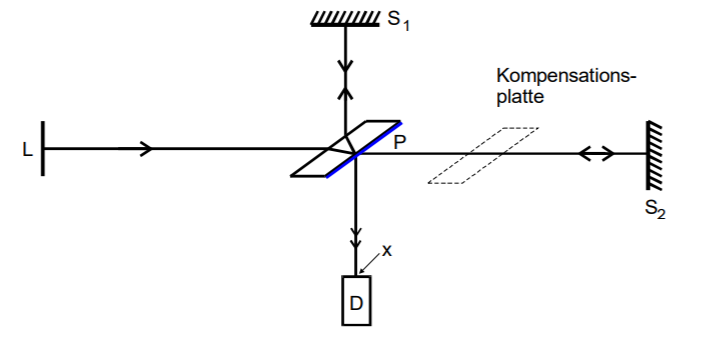
\includegraphics[width=0.4\textwidth]{images/bild2.png}
    \caption{Prinzipieller Aufbau eines Michelson-Interferometers.\cite{V401}}
    \label{fig:bild2}
\end{figure}

Die Lichtquelle $L$ sendet einen Laserstrahl aus, der einen semipermeablen Spiegel $P$ passiert. Dabei wird ein Teil reflektiert und der Andere wird transmittiert.
Beide Strahlen treffen auf einen Spiegel $S_\text{1}$ oder $S_\text{2}$.
Dort werden sie erneut reflektiert und kehren zum Spiegel $P$ zurück. An diesem Spiegel wird theoretisch wieder ein Teil reflektiert und ein Teil transmittiert, jedoch wird nur der Teil betrachtet, der zum Detektor $D$ läuft.
Sind beide Strahlenwege gleich lang, so besitzen die Strahlen eine Verschiebung von $\frac{\lambda}{2}$, wodurch die Intensität verschwindet.
Um die Gleichheit der Wege zu gewährleisten wird auf der Strahlstrecke zu Spiegel $S_\text{2}$ eine Kompensationsplatte befestigt.
Dies wird getan, da der eine Strahl auf dem Weg zum Detektor $D$ drei mal den Spiegel $P$ passiert, und der andere Strahl nur ein mal. 
Beim Passieren des Spiegels $P$ wird der Strahl nämlich gebrochen und es verändert sich die tatsächlich zurückgelegte Weglänge.
Auf diese Weise können die Strahlen angeglichen werden.
Der Spiegel $S_\text{2}$ kann nun um die Länge $\Delta d$ verschoben werden, wodurch sich die Weglänge um $w = 2\Delta d$ ändert.
Gleichzeitig ergibt sich folgender Zusammenhang
\begin{equation}
    \Delta d = \frac{z \cdot \lambda}{2}
    \label{eq:welle}
\end{equation}
$z$ steht für die Anzahl der auftretenden Helligkeismaxima.

Es gibt noch eine weitere Möglichkeit den Wegunterschied zu ändern, so kann ebenfalls auf einem der Strahlenwege ein Medium mit einem anderen Brechungsindex $n' = n + \Delta n$ eingesetzt werden. 
$n$ entspricht hier dem Brechungsgrad der Umgebungsluft.
Das neue Medium wird auf einer Strecke $b$ eingesetzt. 
Der veränderte Aufbau ist schematisch in \autoref{fig:bild3} dargestellt.

\begin{figure}
    \centering
    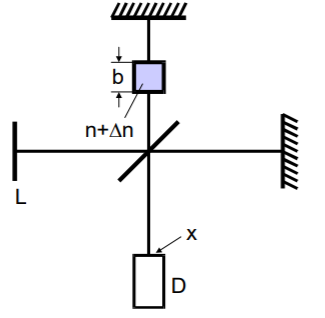
\includegraphics[width=0.4\textwidth]{images/bild3.png}
    \caption{Messung mit dem Michelson-Interferometer durch Brechungsgradunterschiede.\cite{V401}}
    \label{fig:bild3}
\end{figure}

Es lässt sich der Zusammenhang 
\begin{equation}
    b \cdot \Delta n = \frac{z \cdot \lambda}{2}
    \label{eq:f}
\end{equation}
feststellen.

Allgemein gilt ebenfalls
\begin{equation}
    n = \sqrt{1 + f(\lambda)N} \, .
\end{equation}
Wobei $N$ die Anzahl von Molekülen ist, die durch Lichtwellen der Wellenlänge $\lambda$ zu Schwingungen angeregt werden.
Im sichtbaren Bereich des Lichts gilt außerdem für Gase die Näherung
\begin{equation}
    n = 1 + \frac{f(\lambda)}{2} \cdot N.
    \label{eq:n}
\end{equation}
Da angenommen wird, dass sich die verwendeten Gase wie ideale Gase verhalten, kann über die ideale Gasgleichung $pV=RT$ der Zusammenhang
\begin{equation}
    N(p,T) = \frac{p T_0 N_\text{L}}{T p_0}
\end{equation}
hergeleitet werden.
$p_0$ und $T_0$ sind jeweils Druck und Temperatur bei Normalbedingungen und $N_\text{L}$ ist die sogenannte Loschmidt-Konstante.

Nun kann der Druck $p$ innerhalb des Bereiches $b$ auf $p'$ gesenkt werden.
Der Unterschied $\Delta n$ des Brechungsindexes kann dann über den Ausdruck
\begin{equation}
    \Delta n = \frac{f(\lambda)}{2} \cdot N_\text{L} \cdot \frac{T_0}{p_0} \cdot \frac{1}{T} (p - p')
    \label{eq:dn}
\end{equation}
bestimmt werden.
Nun wird \autoref{eq:dn} in \autoref{eq:n} eingesetzt und man erhält unter Normalbedingungen
\begin{equation}
    n = 1 + \Delta n \cdot \frac{T}{T_0} \cdot \frac{p_0}{p-p'} \, .
    \label{eq:n_normal}
\end{equation}
Insgesamt erhält man dann nach einsetzen von \autoref{eq:f} in \autoref{eq:n_normal} für den Brechungsindex des verwendeten Gases
\begin{equation}
    n = 1 + \frac{z \lambda}{2  b } \cdot \frac{T}{T_0} \cdot \frac{p_0}{p - p'}.
    \label{eq:index}
\end{equation}